In the previous sections, we discussed about the anatomy of the brain and neurons and how studies indicate that these cells might communicate via electrochemical pulses known as spikes. We know that sensory input is somehow encoded so that the brain can process it, the exact encoding is not yet known and is the subject of active research effort. Similarly, how is the brain able to reconstruct (or decode) prior input from action potentials is an open question. The so called \emph{neural code} is one of the most important questions in neuroscience and different hypotheses have been proposed, some of which are described bellow~\cite{dayan2001theoretical,gollisch2009throwing}.

\subsection{Rate code}
Spike-rate encoding, in its simplest case, represents information with the amount of action potentials that a neuron generated in a time interval. It is one of the earliest attempts of explaining neural encoding and gives a nice transition from traditional artificial neural networks to spiking ones. Furthermore, there's evidence that neurons that are in direct contact with sensory or motor organs encode information in this way (i.e. the stronger a muscle is flexed, the higher the rate of spikes generated by neurons near muscular tissue).

The main issue with this type of encoding is that it is unable to represent  a large array of different values. For example, if we have a time-slot of $10 ms$ and spikes last $1 ms$, we can only encode 10 values per neuron. Figure \ref{fig:neuro:spike-rate-encoding-cap} shows the case of a $1/10$ rate, no matter when the spike is fired, the encoded value would still be the same.

\begin{figure}[hbt]
  \begin{center}
    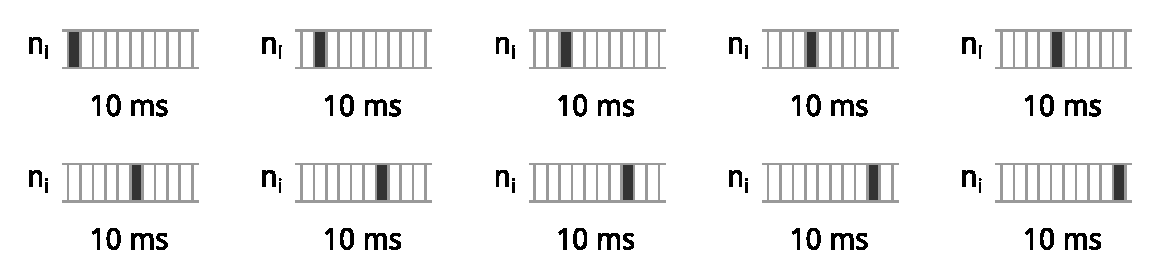
\includegraphics[width=0.8\textwidth]{spike_codes-rate-1}
    \caption{Spike rate example, all 10 combinations encode the same value for they all have a 1 spike per 10 $ms$ rate}
    \label{fig:neuro:spike-rate-encoding-cap}
  \end{center}
\end{figure}

\subsection{Rank-order}
Using this type of encoding, only the temporal order of the spikes generated by a group of neurons is important. It provides more information representation capacity and has been used in computer vision tasks~\cite{rank-order-sparse-memory,basab-model,thorpe-rate-coding-theory}.

\begin{figure}[hbt]
  \begin{center}
    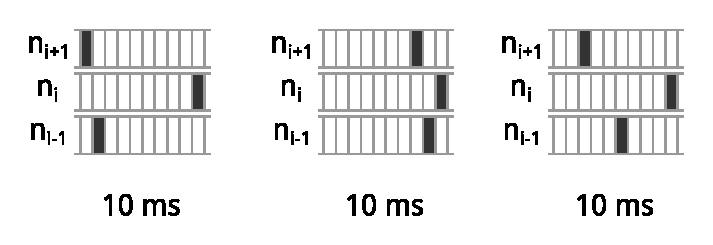
\includegraphics[width=0.55\textwidth]{spike_codes-rank}
    \caption{Rank-order example, since all the examples have neurons firing in the same order, they all encode the same value.}
    \label{fig:neuro:spike-rank-order}
  \end{center}
\end{figure}

An issue that has been noted by some on rank-order encoded information is the fact that spike trains that are notably different (Figure \ref{fig:neuro:spike-rank-order}) are interpreted as the same value. This might be corrected by changing the metrics used to determine the uniqueness of a spike train set~\cite{Cessac2010}. On the other hand, this same issue could be seen as a robust way of encoding information.

\subsection{Temporal code}
The precise time a spike was emitted encodes information. Lots of information, but still difficult to use. Polychronization might be the answer to learning/training.



Input from sensors is most likely rate-based, though processing time and energy consumption in the brain suggests a different one is used for further processing

\subsection{Latency}